\section{Dead Reckoning Localization Method}
\label{sec:2_3_DR}

The American Practical Navigator \cite{bowditch_originally_by_american_2017} defines DR as “a method for determining the estimated position of a vessel by advancing from a known fix of position along the vessel’s ordered course and speed”. 
In this way, maintaining a known course by using the compass and periodically measuring the forward speed, the boats were able to update their last known position frequently, without having to wait for the midday sun to calculate latitude and longitude with the sextant and chronometer.

Therefore, the fundamental characteristic of the DR method is that it is self-contained, that is, it does not require the existence of landmarks or reference points in the environment. 
It is only necessary to know the starting position and the heading and the speed during the integration period. 
In addition, DR also makes it possible to make future projections of the trajectory and, in this way, plan arrival times or avoid obstacles.

However, its main limitation is that, being a relative positioning method based on the last known position, if no corrective measurements are applied, errors accumulate unbounded over time, as depicted in Figure~\ref{fig:DR_error}.
Thus, although the origin of the term is not entirely clear, some theories indicate that ``Dead'' is due to the dangerousness
of such an accumulation of error. Other theories point to the possibility that it was a misspelling from the abbreviation of the term ``Deduced'' \cite{quinion_world_2007}.
% \InsertFig{deadreckoning_method.png}{fig:DR_error}{The Dead Reckoning Method}{The estimate of the position is obtained by updating an initial position using the course and distance traveled in that period. Being a relative method, there is an unbounded accumulation of errors. Source: Paul D. Groves \cite{groves_principles_2008}}{0.9}{}

\begin{figure}[!t]
    \centering
	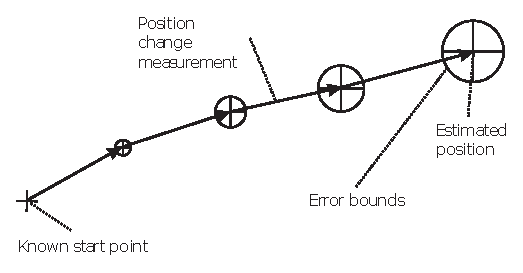
\includegraphics[width=0.8\textwidth]{deadreckoning_method}    	
	\caption[The Dead Reckoning method]{The DR method: the estimate of the position is obtained by updating an initial position using the course and distance traveled in that period. Being a relative method, there is an unbounded accumulation of errors. Source: Paul D. Groves \cite{groves_principles_2008}.}
	\label{fig:DR_error}
\end{figure}
The DR method is not only limited to maritime navigation and can be applied to any mobile element, such as aircraft, land vehicles or mobile robots. In fact, it is known that many mammals use similar path integration techniques to move around the environment.

Depending on the type of moving object, there exist different techniques and technologies for measuring the displacement, speed and course, so diverse as, for example, using a knotted rope for the measuring a boat’s speed  or an odometer for cars and bicycles. 
However, one of the most common technologies nowadays is the use of inertial sensors.
%%%%%%%%%%%%%%%%%%%%%%%%%%%%%%%%%%%%%%%%%%%%%%%%%%%
\subsection{Inertial Navigation Systems}
\label{sec:2_3_1_DR_INS}
Newton's first law of motion defines inertia as the property of bodies to maintain their state of motion, including both the magnitude and direction of their velocity, if no force is applied to them, or if the net force applied to them is null.
Likewise, an inertial reference system is one in which Newton's laws of motion are valid, that is, one that is not accelerated or rotating.

From these concepts arose the idea that, if it were possible to measure the forces acting on a body and trying to change its inertia, it would also be possible to calculate its changes in speed, course and position, regardless of the scenario and condition in which the movement occurs. 
This would be a major advance in the performance of DR-based navigation since, until then, the displacement, speed and course measurements required different techniques and instruments depending on whether the movement was by land, sea or air.

% In the late 19th century, the first inertial sensors capable of measuring angular velocity, known as gyroscopes, appeared. And since the early 20th century, the first accelerometers, capable of measuring linear accelerations.
In the mid-19th century, the first inertial sensors appeared: first, the gyroscopes, capable of measuring angular velocity and, around 70 years later, the accelerometers, capable of measuring linear accelerations.
However, it was not after the World War II, when inertial sensors of sufficient quality became available to construct navigation systems that would enable to track the position, speed and orientation of an object in space for a reasonable period of time and with acceptable accuracy. These systems are known as INS.

% \InsertFig{gimbal.pdf}{fig:gimbal}{Gimbaled INS or stable platform system}{Source: Oliver J. Woodman \cite{woodman_introduction_2007}}{0.5}{}
\begin{figure}[!t]
    \centering
	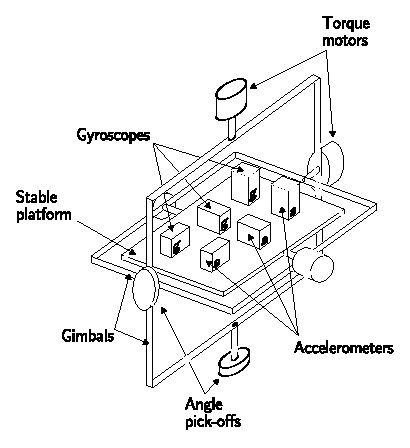
\includegraphics[width=0.6\textwidth]{gimbal}    	
	\caption[Gimbaled INS or stable platform system]{Gimbaled INS or stable platform system. Source: Oliver J. Woodman~\cite{woodman_introduction_2007}.}
	\label{fig:gimbal}
\end{figure}
The early INS used a configuration known as gimbaled INS or stable platform systems: the inertial sensors were mounted on a platform isolated from external rotations by motors that canceled the rotations detected by the gyroscopes, as shown in the Figure~\ref{fig:gimbal}. 
In this way, the accelerometer reference system was kept aligned with the navigation reference system.
%Subsequently, after correcting the value of the gravity on the accelerometers, the speed and position were obtained after successive integrations of the acceleration values.
After correcting the value of the gravity, the speed and position were obtained by successive integrations of the acceleration values.
%(figura~\ref{fig:gimbal_algorithm}).
This architecture was determined by the technological limitation of early gyroscopes and by the need to reduce the computational load that the transformation of accelerations from one reference system to another would imply.
%\InsertFig{gimbal_algorithm.pdf}{fig:gimbal_algorithm}{Gimbaled inertial navigation algorithm}{Source: \cite{woodman_introduction_2007}}{1}{}
Subsequently, with the improved performance of gyroscopes and the availability of increased computing power, a configuration in which inertial sensors were rigidly mounted on the moving object was used. 
This configuration is known as strapdown and, in exchange for greater computational complexity, smaller and mechanically simpler INS are achieved.
Currently, strapdown INS is the most widely used configuration. 

Next, a general description of the implementation of the strapdown INS is presented, introducing the basic types of inertial sensors, an overview of the algorithm formulation and some cumulative error reduction techniques that can be applied so that the system remains self-contained.
There are many references in the literature to these and other aspects of the INS, such as \cite{grewal_global_2001, titterton_strapdown_2004, woodman_introduction_2007, groves_principles_2008, groves_navigation_2015}.
\subsubsection{Inertial Sensors}
\label{sec:2_3_1_1_DR_INS_IMU}
\begin{description}
	\item \textbf{Accelerometers}
	% \InsertFig{accelerometer.pdf}{fig:accelerometer}{Simple mechanical accelerometer}{Source: Paul D. Groves \cite{groves_navigation_2015}}{0.8}{}
	\begin{figure}[!t]
		\centering
		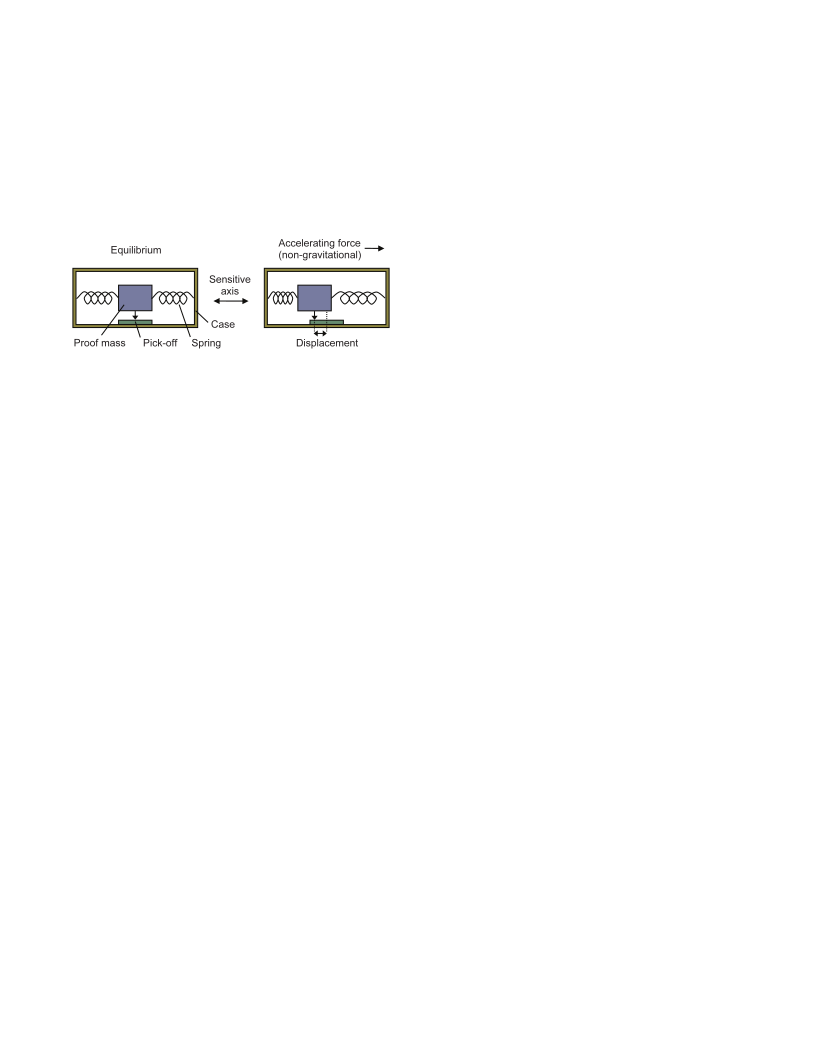
\includegraphics[width=0.8\textwidth]{accelerometer}    	
		\caption[Simple mechanical accelerometer]{Simple mechanical accelerometer. Source: Paul D. Groves \cite{groves_navigation_2015}.}
		\label{fig:accelerometer}
	\end{figure}
	
	In the Figure~\ref{fig:accelerometer} can be seen the structure of a basic mechanical accelerometer.
	The basis of its operation is that the relative position between the test mass of the interior and the case is proportional to the force applied in the direction of the measuring axis. 
	That is, when an acceleration is applied to this axis, the case moves in relation to the test mass through the springs that connect them.
	%Accelerometers only measure non-gravitational accelerations, known as ``specific force'', since accelerations due to gravity affect the entire accelerometer set equally and are not distinguishable.
	%Therefore, if the accelerometer is in free fall, the specific force and, therefore, also the output of the accelerometer will be zero. 	
	Accelerometers only measure non-gravitational accelerations, known as ``specific force''.
	This is because gravity affects the entire sensor and is therefore not distinguishable.
	%This implies that, if the accelerometer is in free fall, the specific force will be zero and therefore the measurement provided by the sensor will also be zero.
	This implies that, if the accelerometer is in free fall, the specific force will be zero and so will be the measurement provided by the sensor.
	On the other hand, if the accelerometer is static and its sensitive axis is parallel to the direction of gravity, the output value of the sensor will be the magnitude of gravity.
	That is why, when integrating accelerations in an INS, it is necessary to know the local value of gravity in order to correct the measurements offered by the accelerometers.	
	Current accelerometers are based on more advanced designs such as pendulums or vibrating beams, built both mechanically and in solid state \cite{titterton_strapdown_2004}.
	
	%%%%%%%%%%%
	%\newpage
	\item \textbf{Gyroscopes}
	
		% \begin{figure}[!t]
			% \centering
			% \subfloat[\textbf{Effect on a ring based gyroscope.}]{
				% 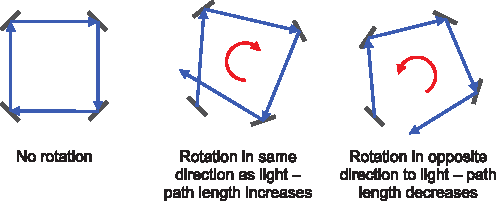
\includegraphics[scale=1.2]{gyro_fiber.pdf}
				% \label{fig:gyro_fiber}}
			% \vfil
			% \subfloat[\textbf{Gyroscope based on a vibrating structure.}]{
				% 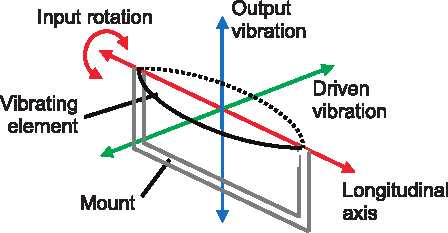
\includegraphics[scale=1]{gyro_vibrating.pdf}
				% \label{fig:gyro_vibrating}}
			% \caption[Working principle of different types of gyroscopes]{Working principle of different types of gyroscopes. Source: Paul D. Groves \cite{groves_navigation_2015}.}
			% \label{fig:MEMS_gyro_types}
		% \end{figure}	
	The first mechanical gyroscopes were based on a spinning wheel mounted on a gimbaled structure, similar to the one shown in Figure~\ref{fig:gimbal}, which allows it to rotate in all three axes.
	Due to the conservation of the angular momentum, the spinning wheel resists to change its orientation and, by reading the pick-offs, the orientation angles can be known.
	%\InsertFig{gyroscope.pdf}{fig:gyroscope}{A conventional mechanical gyroscope}{Source: \cite{woodman_introduction_2007}}{0.5}{}
	
	In contrast, modern gyroscopes offer angular rates instead of orientation angles. 
	They are usually built as fiber optic rings or vibrating structures.
	The former are based on a beam of light emitted through a ring of known length. By measuring the time it takes to go through it, it is possible to know how much the ring turned and in what direction.
	%if the ring has turned, how much it has turned, and in what direction.
	The latter use vibrating elements to measure the Coriolis acceleration and, from it, the angular velocity.
	Diagrams of both types of gyroscopes can be seen in Figure~\ref{fig:MEMS_gyro_types}.	
	%\InsertFig{gyro_fiber.pdf}{fig:gyro_fiber}{Effect on a ring based gyroscope}{Source: \cite{groves_navigation_2015}}{0.8}{}
	%\InsertFig{gyro_vibrating.pdf}{fig:gyro_vibrating}{Gyroscope based on a vibrating structure}{Source: \cite{groves_navigation_2015}}{0.8}{}			
		\begin{figure}[!t]
			\centering
			\subfloat[\textbf{Effect on a ring based gyroscope.}]{
				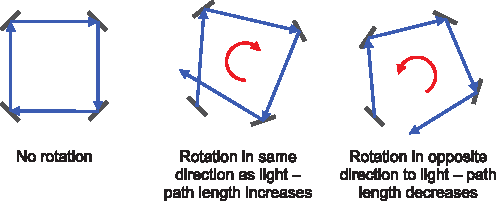
\includegraphics[scale=1.2]{gyro_fiber.pdf}
				\label{fig:gyro_fiber}}
			\vfil
			\subfloat[\textbf{Gyroscope based on a vibrating structure.}]{
				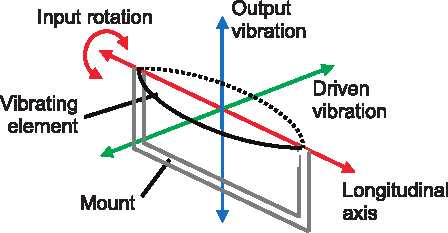
\includegraphics[scale=1]{gyro_vibrating.pdf}
				\label{fig:gyro_vibrating}}
			\caption[Working principle of different types of gyroscopes]{Working principle of different types of gyroscopes. Source: Paul D. Groves \cite{groves_navigation_2015}.}
			\label{fig:MEMS_gyro_types}
		\end{figure}	
	%%%%%%%%%%%
	\item \textbf{Inertial Measurement Units}
	
	A body that can move without restrictions in a three-dimensional space has six degrees of freedom: translations along three perpendicular axes (forward/backward, up/down, left/right) and changes in orientation through rotation about three perpendicular axes.
	Therefore, at least three accelerometers and three gyroscopes will be required to implement an INS in such a scenario.
	
	Accordingly, it is common to group several inertial sensors into a single device, known as \emph{Inertial Measurement Unit} (IMU), which generally contains those three accelerometers and three gyroscopes placed in orthogonal directions.
	In addition, IMUs may contain additional sensors, such as magnetometers and barometers, and signal matching and calibration capabilities, power supply and communication interfaces.	
	%%%%%%%%%%%%
	\item \textbf{Inertial Sensors' Errors}
	
	Inertial sensors are not perfect devices and have different types of errors. These are some of the most important:
	\begin{itemize}
		\item Bias: It is the offset between the measurement and the actual value. It is usually the biggest source of error.
		\item Scale-factor: This is the separation between the ratio of actual to estimated values and the unit slope line. That is, it indicates whether the error is proportional to the value of the measured variable. 
		\item Cross-coupling: This occurs when the physical quantities produced in one axis are ``felt'' on other perpendicular axes of the sensor. This is usually due to misalignment during sensor construction.
		\item Random errors: They are due to mechanical and electrical sources. Usually known as ``random walk'' because of the effect of its integration.
	\end{itemize}	
	
	The first three types of errors are systematic and are made up of four fundamental components:
	\begin{itemize}
		\item Fixed contribution: Present each time the sensor is used.
		\item Effect of temperature: Temperature changes affect sensor response.
		\item Run-to-run variation: It is the variation of each error source between different uses of the sensor.
		\item In-run variation: It is the variation of each error source during one use of the sensor.
	\end{itemize}
	The first two error components can be eliminated or reduced through calibration processes. 
	Not the latter two, which can only be corrected by the use of external information.	
	This way, an error model of the IMU's accelerometers can be written:
	\begin{equation}
	\label{eqn_acc_error}
		\boldsymbol{\hat{f}}=\boldsymbol{b_a}+(\boldsymbol{I_3}+\boldsymbol{M_a})\boldsymbol{f}+\boldsymbol{w_a}
	\end{equation}	
	where $\boldsymbol{\hat{f}}$ is the specific force vector measured by the IMU's accelerometers, $\boldsymbol{b_a}$ the accelerometers' bias vector, $\boldsymbol{I_3}$ is the identity matrix, $\boldsymbol{M_a}$ is the matrix of the coefficients of the accelerometers scale-factor (diagonal elements) and cross-coupling errors (off-diagonal elements), $\boldsymbol{f}$ is the true specific force vector and $\boldsymbol{w_a}$ is the random-noise vector.
	And similarly for gyroscopes:
	\begin{equation}
	\label{eqn_gyr_error}
		\boldsymbol{\hat{\omega}}=\boldsymbol{b_g}+(\boldsymbol{I_3}+\boldsymbol{M_g})\boldsymbol{\omega}+\boldsymbol{G_g}\boldsymbol{f}+\boldsymbol{w_g}
	\end{equation}		
	where $\boldsymbol{\omega}$ is referred to the angular rate, $\boldsymbol{G_g}$ is the matrix of errors dependent on the accelerations suffered by the gyroscopes, and the rest of symbols are analogous to the accelerometer case.
	%%%%%%%%%%%%
	\item \textbf{MEMS Technology}	
	
	Among the different types of gyroscopes and accelerometers available, the best performances are usually associated with those of greater size and mechanical complexity.
	This has consequences in terms of usability, as it impacts on their portability and cost, for example.
		
	Since the end of the 20th century, the development of the MEMS technology has made it possible to develop small, lightweight, low-cost inertial sensors. 
	This has allowed them to be included in a multitude of portable devices, such as smartphones or wearable devices, and, therefore, to be available for pedestrian applications.
	However, although its performance continues to improve, this reduction in size leads to higher levels of error, as shown in Figure~\ref{fig:MEMS_performance}.	
	It is therefore common for inertial sensors to be classified according to their accuracy in categories such as marine, aviation, tactical or consumer.			
	\begin{figure}[!t]
		\centering
		\subfloat[\textbf{Accelerometers}]{
			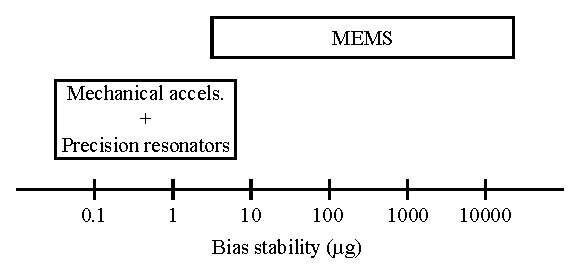
\includegraphics[]{MEMS_acc}
			\label{fig:MEMS_acc}}
		\vfil
		% \subfloat[\textbf{Accelerometers}]{
			% 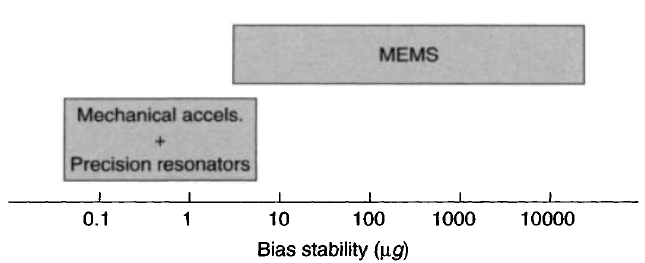
\includegraphics[width=0.8\textwidth]{MEMS_acc_old.png}
			% \label{fig:MEMS_acc}}
		% \vfil		
		\subfloat[\textbf{Gyroscopes}]{
			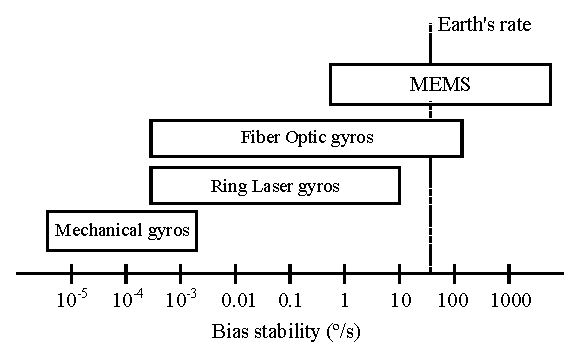
\includegraphics[]{MEMS_gyro}
			\label{fig:MEMS_gyro}}
		% \subfloat[\textbf{Gyroscopes}]{
			% 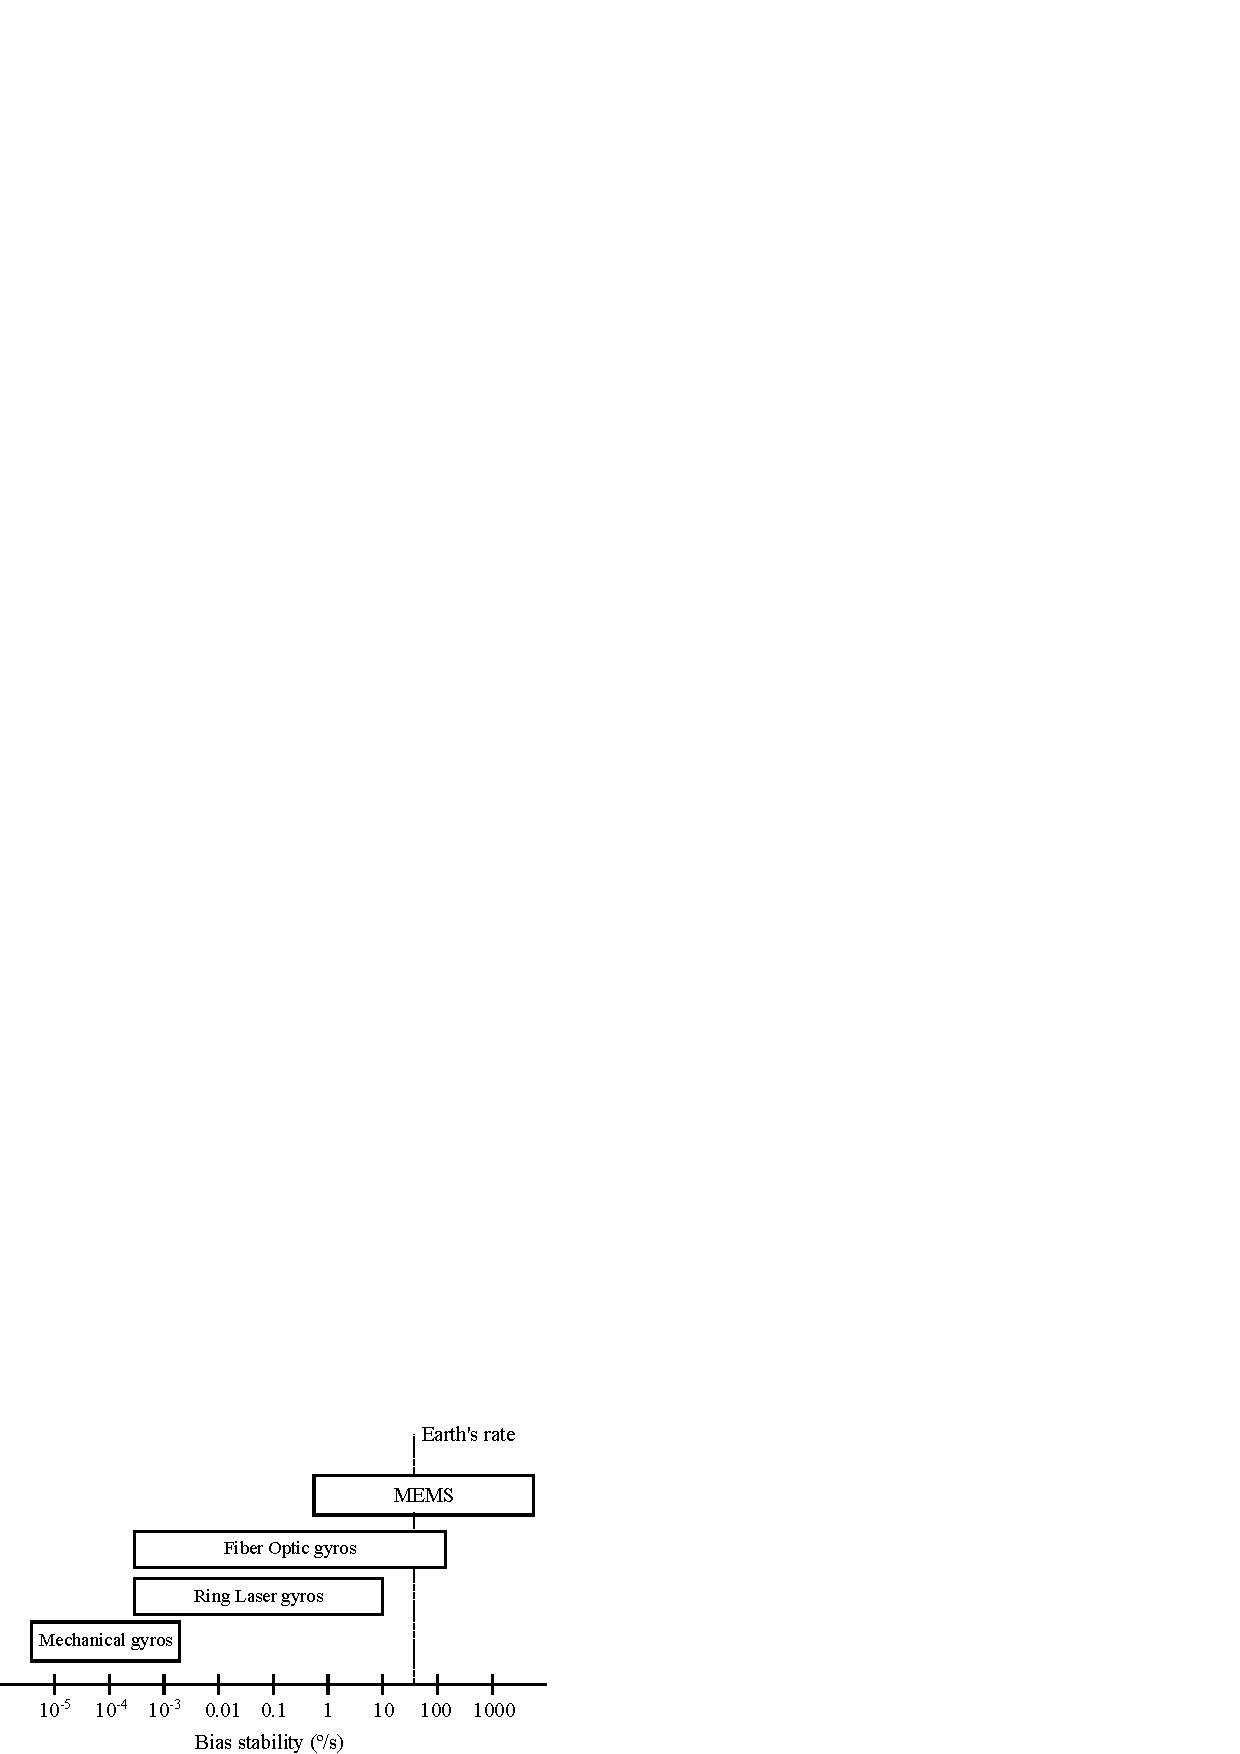
\includegraphics[width=0.8\textwidth]{MEMS_gyro.png}
			% \label{fig:MEMS_gyro}}			
	    \caption[Performance comparison of different types of inertial sensors]{Performance comparison of different types of inertial sensors. Source: D.H. Titterton and Weston\cite{titterton_strapdown_2004}.}
		\label{fig:MEMS_performance}
	\end{figure}	
\end{description}

\subsubsection{Strapdown INS Mechanization}
\label{sec:2_3_1_2_DR_INS_SINS}
The following will briefly explain the fundamental steps of the strapdown INS algorithm. 
There are different variants of this method, known as mechanizations, depending on which system is chosen as reference frame.
In this case it will be considered that navigation is required with respect to a fixed reference frame. That is, an inertial reference system, which is neither rotating nor accelerated.

A fixed reference system in relation to the Earth is not inertial, as the planet rotates and moves through the universe.
Since accelerometers and gyroscopes provide measurements with respect to an inertial system, the rotations and the accelerations associated with the Earth's movement (centripetal, Coriolis and Euler) should be taken into account when navigating with respect to the it.
However, if we limit ourselves to the case of pedestrians and MEMS-based IMUs, the low speed at which we walk and the noise levels of the sensors (as can be seen in the Figure~\ref{fig:MEMS_gyro}) allow to assume that the Earth is a fixed reference frame.

Throughout this section, the subscripts b (body frame) and g (global frame) are used to indicate the frame of reference in which vector quantities are measured, as can be seen in the Figure~\ref{fig:body_reference}.
% \InsertFig{body_reference.pdf}{fig:body_reference}{The body and global frames of reference}{Source: Oliver J. Woodman \cite{woodman_introduction_2007}}{0.5}{}
\begin{figure}[!t]
    \centering
	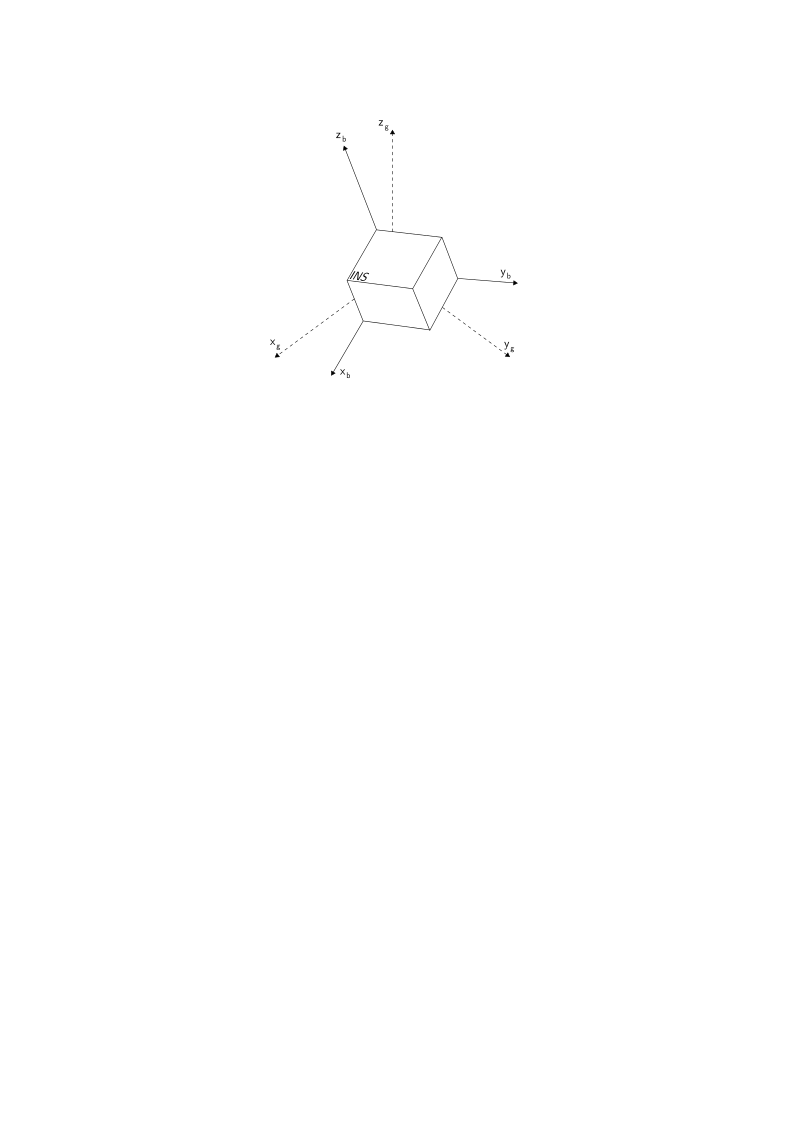
\includegraphics[width=0.5\textwidth]{body_reference}    	
	\caption[The body and global frames of reference]{The body and global frames of reference. Source: Oliver J. Woodman~\cite{woodman_introduction_2007}.}
	\label{fig:body_reference}
\end{figure}

The strapdown INS mechanization can be divided into 4 basic steps: orientation update, accelerations projection, gravity correction and integration.

Knowing the orientation of the moving object with respect to the global frame is necessary for several reasons.
On the one hand, because it is essential for later projecting the accelerations from the body frame to the global frame before integrating them;
And, on the other hand, because, in general, orientation cannot be assumed from the direction of traveling. 
Think, for example, of a person walking sideways: the direction in which he looks does not coincide with that of his displacement.

There are different ways to represent orientations.
Some of the most common ones are rotation matrices, Euler angles and quaternions \cite{shuster_survey_1993}. 
In this case, we will use rotation matrices.	
It can be shown that, using the small angle approximation, the variation over time of a rotation matrix can be expressed by the following differential equation (\cite{titterton_strapdown_2004, woodman_introduction_2007}):
\begin{equation}
\label{eqn_dcm_ed}
	\boldsymbol{\dot{C}}(t)=\boldsymbol{C}(t)\boldsymbol{\Omega}(t)
\end{equation}	
which has the solution:
\begin{equation}
\label{eqn_dcm_ed_sol}
	\boldsymbol{C}(t)=\boldsymbol{C}(0)\cdot exp \left( \int_{0}^{t}\boldsymbol{\Omega}(t) dt \right)
\end{equation}		
where
\begin{equation}
\label{eqn_skew_matrix}
	\boldsymbol{\Omega}(t)=
	\begin{pmatrix}
		0&-\omega_{bz}(t)&\omega_{by}(t)\\
		\omega_{bz}(t)&0&-\omega_{bx}(t)\\
		-\omega_{by}(t)&\omega_{bx}(t)&0
	\end{pmatrix}		
\end{equation}	
is the skew symmetric form of the angular rate vector $\omega_b(t)$.

Since most gyroscopes are digital and they provide angular rate values periodically ($\triangle t$), it can be shown that the orientation update equation after each successive gyroscope sample has the following form:
\begin{equation}
\label{eqn_dcm_update}
	\boldsymbol{C}(t+\triangle t)=\boldsymbol{C}(t) \left( \boldsymbol{I}+\frac{\sin \sigma}{\sigma}\boldsymbol{B}+\frac{1-\cos\sigma}{\sigma^2}\boldsymbol{B}^2 \right)
\end{equation}
where $\sigma=|\omega_b\triangle t|$ and the matrix $\boldsymbol{B}$:
\begin{equation}
\label{eqn_skew_matrix_upd}
	\boldsymbol{B}=
	\begin{pmatrix}
		0&-\omega_{bz}\triangle t&\omega_{by}\triangle t\\
		\omega_{bz}\triangle t&0&-\omega_{bx}\triangle t\\
		-\omega_{by}\triangle t&\omega_{bx}\triangle t&0
	\end{pmatrix}		
\end{equation}	

These expressions assume infinitesimal rotations and sampling periods. Therefore, the sampling frequency of gyroscopes should, in general, be as high as possible, so that the angular velocity can be considered as constant between each measurement period.

Once the current orientation of the object is obtained, it is possible to project the accelerations from the IMU's body frame to the global frame:
\begin{equation}
\label{eqn_acc_proy}
	\boldsymbol{a}_g(t)=\boldsymbol{C}(t)\boldsymbol{a}_b(t)
\end{equation}
where $\boldsymbol{a}_b(t)=(a_{bx}(t),a_{by}(t),a_{bz}(t))^T$ are the measurements from the accelerometers.

Finally, the only thing left to do is to correct the gravity, expressed in global frame ($\boldsymbol{g}_g$), and carry out the successive integrations.
In a similar way to gyroscopes, the accelerometers deliver their measurements periodically, so integrating by the rectangular rule, the update equations will be:
\begin{equation}
\label{eqn_acc_int}
	\boldsymbol{v}_g(t+\triangle t)=\boldsymbol{v}_g(t)+\triangle t \cdot (\boldsymbol{a}_g(t+\triangle t)-\boldsymbol{g}_g)
\end{equation}
\begin{equation}
\label{eqn_vel_int}
	\boldsymbol{s}_g(t+\triangle t)=\boldsymbol{s}_g(t)+\triangle t \cdot (\boldsymbol{v}_g(t+\triangle t))
\end{equation}
where $\boldsymbol{v}_g(t)$ y $\boldsymbol{s}_g(t)$ are the velocity and position of the moving body, expressed in the global frame, at time $t$.
A general diagram of the algorithm just explained can be seen in the Figure~\ref{fig:strapdown_algorithm}.
% \InsertFig{strapdown_algorithm.pdf}{fig:strapdown_algorithm}{Strapdown INS mechanization for a fixed reference frame}{Source: Oliver J. Woodman \cite{woodman_introduction_2007}}{1}{}
\begin{figure}[!t]
    \centering
	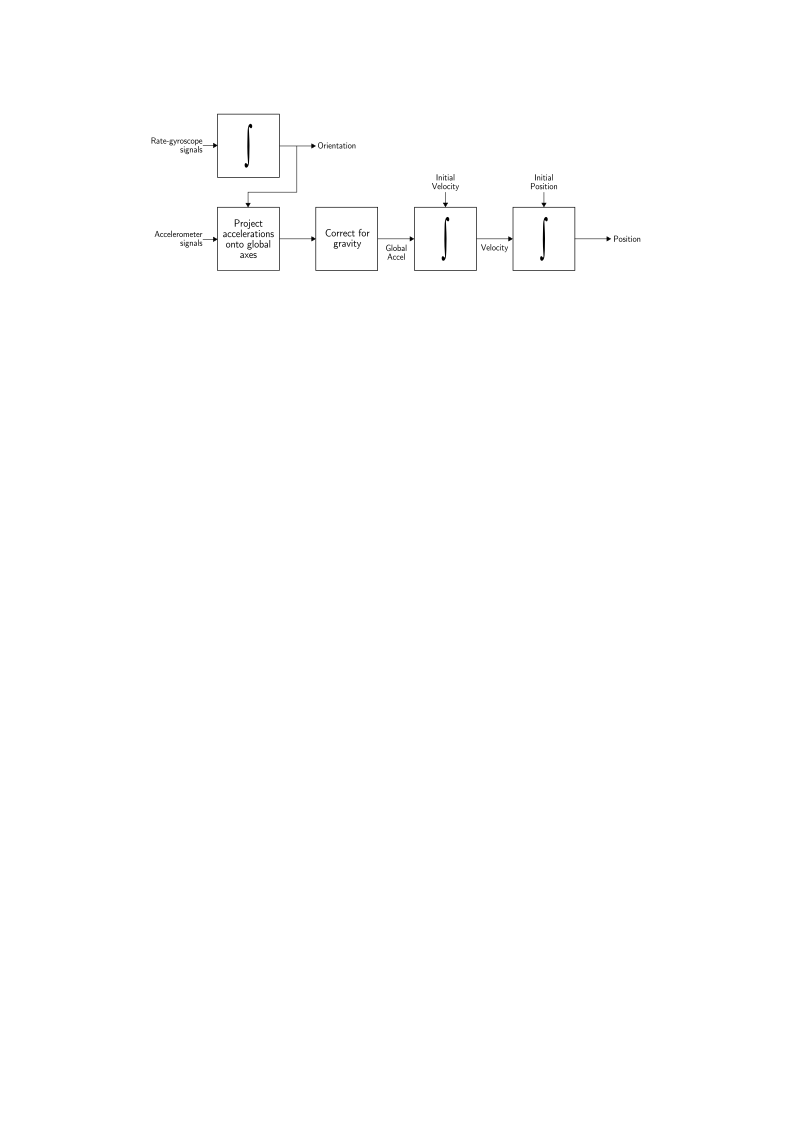
\includegraphics[width=1\textwidth]{strapdown_algorithm}    	
	\caption[Strapdown INS mechanization for a fixed reference frame]{Strapdown INS mechanization for a fixed reference frame. Source: Oliver J. Woodman~\cite{woodman_introduction_2007}.}
	\label{fig:strapdown_algorithm}
\end{figure}
\subsubsection{Drift Reduction Techniques}
\label{sec:2_3_1_3_DR_INS_ZUPT}
As discussed in Section~\ref{sec:2_3_1_1_DR_INS_IMU}, inertial sensors contain errors and, since strapdown INS is an integration-based method, those errors will also be integrated and will accumulate unbounded over time.
On the one hand, the errors of the gyroscopes will propagate as orientation errors when integrated, which will grow proportionally with time.
On the other hand, the errors of the accelerometers will propagate linearly in time as velocity errors and, after the second integration, as position errors in a quadratic rate.
However, the orientation error also propagates as position error since it causes that the projection of the accelerations is done wrongly and, therefore, the correction of gravity as well.
Therefore, the total position error grows cubically in time.
%In fact, for many applications that orientation error is critical, since the magnitude of the gravity can be much greater than the average accelerations that the object undergoes, reason why any small error of orientation will have a great impact in the position error .
%In fact, for many applications, this orientation error is critical: When the magnitude of the gravity can be much greater than the average accelerations that the object undergoes, any small orientation error will have a great impact in the position error .
%De hecho, debido a la magnitud de la gravedad, cualquier pequeño error de orientación puede generar un error de posición mayor que el debido a los errores de los acelerómetros.
In fact, orientation error is critical: due to the magnitude of the gravity on Earth, any small orientation error will have a great impact in the position error.

The position error accumulation is especially evident if inertial sensors based on MEMS technology are used.
In the Figure~\ref{fig:MEMS_error_position} the position error accumulation rate for a static strapdown INS using a medium-low cost IMU is shown.
As can be seen, this position error rate makes navigation unfeasible after a few seconds.
Therefore, the use of INS systems based on MEMS IMUs, which are the most convenient for pedestrians, seems complicated.
And, in general, although high precision inertial sensors are used, the use of INS is limited in time.
% \InsertFig{MEMS_error_position.pdf}{fig:MEMS_error_position}{Average drift position when applying strapdown INS to a static MEMS-based IMU's measurements}{Source: Oliver J. Woodman \cite{woodman_introduction_2007}}{1}{}
\begin{figure}[!t]
    \centering
	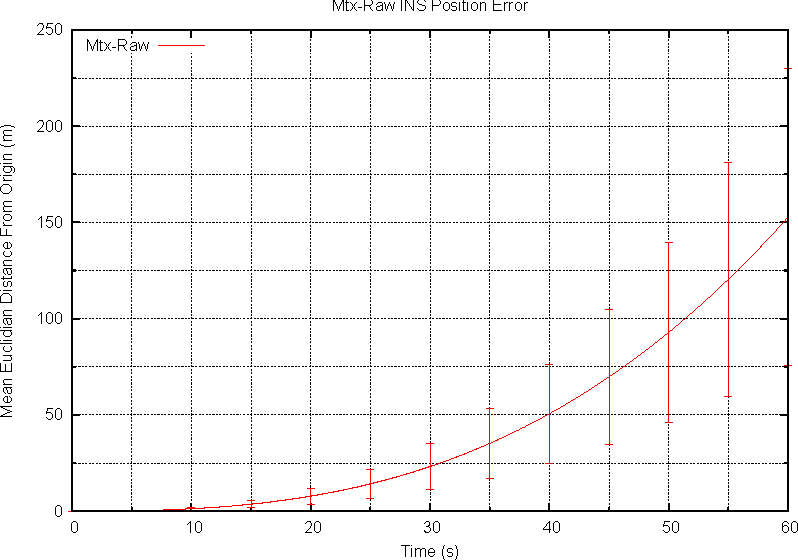
\includegraphics[width=1\textwidth]{MEMS_error_position}    	
	\caption[Average drift position of a static strapdown INS with a MEMS-based IMU]{Average drift position of a static strapdown INS with a MEMS-based IMU. Source: Oliver J. Woodman~\cite{woodman_introduction_2007}.}
	\label{fig:MEMS_error_position}
\end{figure}
However, as will be seen in the following Section~\ref{sec:2_4_fusion}, by merging with other technologies and additional information sources, it is possible to use INS systems in such a way that they are useful for navigation.
%Among the different types of information that can be merged, in this section we will highlight those that allow the system to remain self-contained:
Among the different types of information that can be merged, those that allow the system to remain self-contained are now introduced.
\begin{description}
	\item \textbf{A priori knowledge about object's dynamic}
	
	The knowledge about the characteristics of the movement of an object can give the possibility of identifying scenarios in which the value of some of the variables describing its movement is known a priori and, therefore, some corrections can be applied under that assumption.

	One of the most common corrections are the ZUPT, which consist in detecting the moments in which it is known that the object is still. This allows to correct the value of the estimated velocity at that moment. In this way, the rate of accumulation of the velocity and position error is reduced, providing a longer operation time the INS.

	Another corrective measure is the one known as \emph{Zero-Angular Rate Updates} (ZARU), which, likewise, consists of detecting the static moments of the object but, in this case, to estimate the value of the gyroscopes' bias, since it can be assumed that their output values should be zero at those moments. In this way, the growth rate of the orientation error is reduced, which also impacts the estimation of the velocity and position.
	
	These techniques have been successfully applied to different scenarios, such as underwater navigation \cite{huddle_trends_1998}, oil drilling \cite{ledroz_fog-based_2005} or geographic mapping \cite{grejner-brzezinska_bridging_2001}, and, thanks to the characteristics of the human gait, it can also be applied to pedestrians.
	Through the use of foot-mounted IMUs, it is possible to detect the moments when the foot is still on the ground, which occurs periodically at each footstep.
	In this way, it is possible to periodically correct INS errors and reduce the accumulation of the position error to a rate proportional to the number of strides.
	Furthermore, the detection of the stance periods is possible using only the acceleration and angular rate signals, so the system remains self-contained.
	With this solution, position errors close to 1\% of the traveled distance can be achieved using MEMS IMUs, surpassing even ``pure'' INS systems with higher performance IMUs.
	The work of Eric Foxlin is recognized for being the first to use efficiently the ZUPT technique for foot-mounted IMUs \cite{foxlin_pedestrian_2005}, and a good explanation can also be found in the work of Jiménez \emph{et al.} \cite{jimenez_indoor_2010}.	
	%%%%%%%%%%%%%%%%%%%%%%%%%%%%%%%%%%%
	\item \textbf{Use of magnetometers}
		
	With techniques such as ZUPT and ZARU it is possible to reset velocity and position errors, estimate accelerometer and gyroscope biases and even correct tilt-related orientation errors.
	However, the heading error is not observable and is therefore currently the main limitation of the INS systems.
	
	One of the most common solutions is the use of magnetometers, by means of which it is possible to calculate the direction of the magnetic north and, in this way, the heading error can be corrected. In addition, it also allows the system to remain self-contained.
	
	Unfortunately, their use is restricted to outdoors scenarios, since the presence of metallic and electrical elements in buildings and different constructions cause distortions in the magnetic field, making the use of magnetometers unreliable as a measurement of the actual heading value.		
\end{description}	
%%%%%%%%%%%%%%%%%%%%%%%%%%%%%%%%%%%%%%%%%%%%%%%%%%%
\subsection{Pedestrian Dead Reckoning Systems}
\label{sec:2_3_2_DR_PDR}
\begin{figure}[!t]
	\centering
	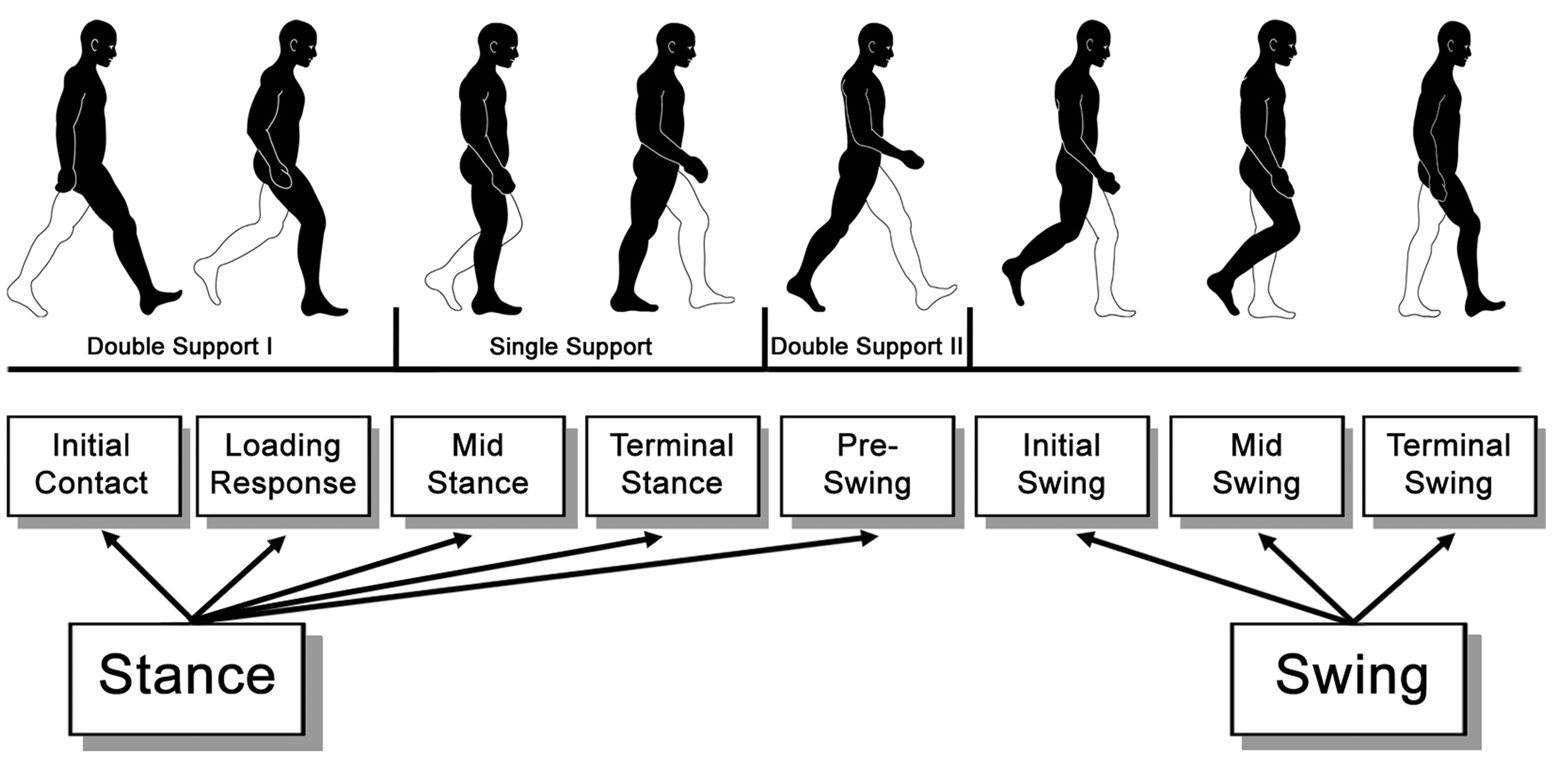
\includegraphics[width=\textwidth]{gait_cycle_cut}
	\caption[Functional divisions of the gait cycle]{Functional divisions of the gait cycle: the gait cycle or stride has two phases. The stance phase is that part during which the reference foot remains in contact with the ground. It constitutes 60 percent of the gait cycle and includes five moments: the initial contact (Heel Strike), the loading response (Foot Flat), the mid and terminal stance, and the pre swing (Toe Off). The swing phase is rest of the gait cycle during which the reference foot swings in the air. Source: T. Stöckel \emph{et .al} \cite{stockel_mental_2015}.}
	\label{fig:GaitCycle}
\end{figure}
%\InsertFig{gait_cycle}{fig:GaitCycle}{Functional divisions of the gait cycle}{A gait cycle consists of two main phases – the stance and swing phase – and eight functional periods. Source: \cite{stockel_mental_2015}}{1}{}
Walking is the most common form of human locomotion and is based on the continuous repetition of a series of movements of different parts of the body, especially the lower limbs.
From the different phases through which the foot passes, a pattern known as gait cycle or stride is defined.
As can be seen in the Figure~\ref{fig:GaitCycle}, a stride is defined between two consecutive moments in which a foot (by convention, the right one) begins the contact with the ground.
During the gait cycle, the forward movement basically consists of moving one leg forward while the weight of the body is supported on the opposite leg, which has the foot resting on the ground.

The gait cycle is usually characterized by a set of gait parameters including the stride length and step length.
%These two gait parameters are close related: As can be seen in the Figure~\ref{fig:step_stride_description_2}, the stride length is defined between the positions of two consecutive footfalls of the same foot, while the step length is defined between opposite feet and measured in the forward direction.
These two gait parameters are close related: the stride length is defined between the positions of two consecutive footfalls of the same foot, while the step length is defined between opposite feet and measured in the forward direction.
In fact, when walking straight and without anomalies, the stride lengths of both feet are equal and each stride length is equal to the sum of the last two step lengths.
%\InsertFig{step_stride_description_2}{fig:step_stride_description_2}{Stride length and step length.}{Stride length is defined between the positions of two consecutive footfalls of the same foot, while the step length is the distance between opposite feet and measured in the forward direction.}{1}{}
%\InsertFig{step_stride_description_2}{fig:step_stride_description_2}{Stride length and step length.}{}{0.8}{}

The basic idea of the PDR technique is to adapt the DR method to the human walking fundamental characteristics, that is, to the gait cycle.
Since walking occurs mostly on a usually level plane, PDR systems limit the estimation of the position to the two-dimensional case, expressing the trajectory of a person as a concatenation of stride lengths, as shown in Figure~\ref{fig:PDR_decomposition}.
This way, the position update after the k-th stride can be written as follows:
\begin{equation}
\label{eqn_SHS}
	\begin{aligned}
	X(k)&=X(k-1)+SL(k)\cdot \cos(\psi(k))\\
	Y(k)&=Y(k-1)+SL(k)\cdot \sin(\psi(k))
	\end{aligned}
\end{equation}
where $SL(k)$ y $\psi(k)$ are the stride's length and heading angle, respectively.
Similarly, the position update can also be expressed using steps instead of strides.
%\InsertFig{PDR}{fig:PDR_decomposition}{A pedestrian trajectory expressed as a concatenation of strides, through their length and orientation.}{Figure adapted from \cite{zampella_localizacion_2017}}{0.8}{}
\begin{figure}[!t]
	\centering
	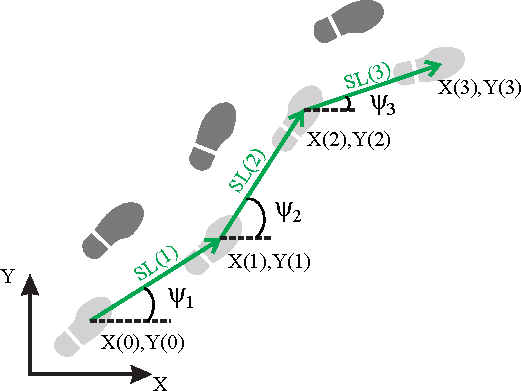
\includegraphics[width=0.8\textwidth]{PDR}
	\caption[A pedestrian trajectory expressed as a concatenation of strides]{A pedestrian trajectory expressed as a concatenation of strides, through their length and orientation. Figure adapted from Francisco Zampella \cite{zampella_localizacion_2017}.}
	\label{fig:PDR_decomposition}
\end{figure}
This formulation based on gait parameters makes the PDR systems to usually be composed of three main blocks: SD, SLE and SHE.
%As it was mentioned in chapter~\ref{cha:1_Introduction}, these systems are also known as step-and-heading systems (SHS) \cite{harle_survey_2013}.

Sometimes, information about the altitude is also necessary. This is the case inside buildings, where knowing the floor may be sufficient. This is usually known as 2.5 dimensional positioning.

% Aunque la definición de muchos de los gait parameters está basada en la posición y movimiento de los pies (entre ellos step length y stride length), la estructura mecánica del cuerpo humano implica que tanto las causas como los efectos del gait cycle estarán distribuidos a lo largo de las diferentes partes del cuerpo.
% Esto significa que deben existir relaciones entre las señales observadas en diferentes partes del cuerpo y los diferentes gait parameters.
% Por tanto, el conocimiento de dichos modelos permitiría diseñar sub-algorithms PDR específicamente diseñados para obtener la longitud y heading de los steps/strides desde  partes del cuerpo específicas.
% Esta es la principal fortaleza de los sistemas PDR: gracias a la naturaleza mecánica del cuerpo humano, los sistemas PDR son flexibles en relación al punto de montaje de los sensores, mejorando así su usabilidad.

% Sin embargo, la obtención de dichos modelos no suele ser sencilla y habitualmente se recurre a modelos biomecánicos o a técnicas de aprendizaje estadístico que obtienen modelos aproximados a partir del análisis previo de un conjunto reducido de instancias del gait cycle.
% Por tanto, la principal debilidad de los sistemas PDR es una falta de generalizabilidad que hace que su rendimiento decrezca cuando las características del movimiento o del subject difieran de los patrones usados durante la creación de los modelos.

Although the definition of many of the gait parameters is based on the position and movement of the feet (including the step length and stride length), the mechanical structure of the human body implies that both the causes and effects of the gait cycle will be distributed throughout different parts of the body.
This means that there must be relationships between the signals observed in different parts of the body and the different gait parameters.
Therefore, the knowledge of such models would allow to design the PDR blocks capable of obtaining the length and heading of the steps/strides from specific body parts.
This is the main strength of PDR systems: thanks to the mechanical nature of the human body, PDR systems are flexible in relation to the mounting point of the sensors, thus improving their usability.

However, obtaining such models is not easy and usually involves biomechanical models or statistical learning techniques. 
In both cases, they obtain approximate models from a previous analysis of a reduced set of instances of the gait cycle.
Therefore, the main weakness of PDR systems is a lack of generalizability that causes their performance to decrease when the characteristics of the motion or the user differ from the patterns used during model creation.

PDR systems can be implemented using different technologies. Some examples include electromyography sensors attached to the calf \cite{wang_novel_2010}, ultrasonic ranging between the feet \cite{saarinen_personal_2004} or the combination of force sensor and ultrasonic transceivers \cite{yeh_geta_2007}.
However, inertial sensors remain the most common technology for the implementation of PDR systems. 
Especially those based on MEMS technology, thanks to their cost, size, weight and their integration in many electronic devices in the market.

% En resumen, para el caso particular de pedestrians y MEMS-based IMUs, INS es el método general y más potentes pero, debido a la calidad de los sensores actuales, la única implementación factible requiere de la utilización de correcciones ZUPT y, por tanto, foot-mounted sensors.
% Por contra, los sistemas PDR ofrecen un interesante compromiso entre usabilidad y adaptabilidad: permiten una mayor flexibilidad en cuanto al punto de montaje del sensor pero su funcionamiento suele estar limitado a un conjunto finito de movimientos (commonly, forward walking and bidimensional positioning) y tipos de usuario.
% Mientras no aumente la calidad de los sensores inerciales para permitir la utilización de INS en más situaciones, los sistemas PDR pueden ser interesantes y suficientes para muchas aplicaciones.

In summary, for the particular case of pedestrians and MEMS-based IMUs, INS is the general and more powerful method but, due to the current quality of that type of sensors, the only feasible implementation requires the use of ZUPT corrections and, therefore, foot-mounted sensors.
In contrast, PDR systems offer a compromise between usability and adaptability: they allow greater flexibility in terms of the sensor's mounting point but their operation is usually optimized to a finite set of motions (commonly, forward walking and two-dimensional positioning) and user's characteristics.
In addition, for both types of systems, the position error is proportional to the number of steps.
For these reasons, as long as the quality of inertial sensors does not increase to allow the use of INS in more situations, PDR systems can be interesting and sufficient for many applications and use cases.

Since inertial PDR systems are the framework for this research work, the following Chapter~\ref{cha:3_pdr_sota} will focus exclusively on reviewing the state of the art of this type of localization systems.